\documentclass[letterpaper, 11pt]{extarticle}

\input{preamble}
\input{format}
\input{commands}

% Listings style for code
\lstset{
    language=Python,
    basicstyle=\ttfamily\small,
    keywordstyle=\color{blue},
    commentstyle=\color{gray}\itshape,
    stringstyle=\color{red},
    showstringspaces=false,
    numbers=left,
    numberstyle=\tiny\color{gray},
    numbersep=8pt,
    breaklines=true,
    frame=single,
    backgroundcolor=\color{gray!5},
}

\begin{document}

\begin{Large}
    \textsf{\textbf{CS361 - HW2}}
\end{Large}

\vspace{1ex}

\textsf{\textbf{Student:}} \text{Shrey Poshiya}\\

Github Link: https://github.com/sposhiy33/CS361HW

\vspace{2ex}


% Problem 1 - Towers of Hanoi
\begin{problem}{}{problem-1}
    In the classic problem of the \textbf{Towers of Hanoi}, you have 3 towers/rods and $n$ disks of different sizes which can slide onto any tower. The puzzle starts with disks sorted in ascending order of size from top to bottom (i.e., each disk sits on top of an even larger one). You have the following constraints:
    \begin{enumerate}
        \item Only one disk can be moved at a time.
        \item A disk is slid off the top of one tower onto another tower.
        \item A disk cannot be placed on top of a smaller disk.
    \end{enumerate}
    Write a recursive solution that prints every individual move in the format: \texttt{"Move disk X from Tower A to Tower C"}, and analyze the time complexity of your algorithm.
\end{problem}

\vspace{1ex}
\noindent\textbf{Implementation:}
\lstinputlisting[language=Python,caption={Tower of Hanoi (\texttt{problem1.py})}]{../HW2/problem1.py}

\vspace{0.5ex}
\noindent\textbf{Sample output:}
\begin{lstlisting}[numbers=none, frame=single, basicstyle=\ttfamily\small]
move disk 1 from A to C
move disk 2 from A to B
move disk 1 from C to B
move disk 3 from A to C
move disk 1 from B to A
move disk 2 from B to C
move disk 1 from A to C
\end{lstlisting}


\textbf{Time Complexity Analysis:} at every step of this recusion, we make two recurive calls, where each call is made to the $n-1$ disks aobve the $n$th disk. Therefore, when we get to the top disk, it's level in the recursive tree will have $2^n$ nodes. The next disk, will have $2^{n-1}$ nodes, and so on. Therefore, the total number of nodes (which is essentially the number of steps) in the recursive tree is: $2^n + 2^{n-1} + ... + 2^1 + 2^0$. Therefore, $$ O(2^n + 2^{n-1} + ... + 2^1 + 2^0) = O(2^n)$$


% Problem 2 - Hybrid Sort
\begin{problem}{}{problem-2}
    You've learned that merge sort has $O(n \log n)$ time complexity, but it has overhead from recursive calls. For small arrays, simpler algorithms like insertion sort can actually be faster.

    \vspace{1ex}
    \noindent\textbf{Part A --- Implementation:}

    Implement a hybrid sort that uses merge sort for large subarrays but switches to insertion sort when the subarray size falls below a threshold $k$.

    \vspace{1ex}
    \noindent\textbf{Part B --- Experimentation and Analysis:}
    \begin{enumerate}
        \item Choose at least 3 different array sizes of your own between 100 and 10,000 (for example: 500, 2000, 8000). Pick sizes that run comfortably on your laptop.
        \item For each array size, run your hybrid sort with $k$ values of $1, 2, 4, 8, 16, 32, 64$.
        \item For each combination of $(n, k)$, repeat the sort 5 times on freshly generated random arrays and record the average runtime in milliseconds.
        \item Plot your results with:
        \begin{itemize}
            \item X-axis: threshold value $k$
            \item Y-axis: average runtime in milliseconds
            \item One curve per array size on the same plot
        \end{itemize}
        \item Identify the optimal value of $k$ (lowest runtime) for each array size from your plot.
        \item Explain why an optimal threshold exists, specifically, why both very small and very large values of $k$ lead to worse performance.
    \end{enumerate}
\end{problem}

\begin{figure}[H]
    \centering
    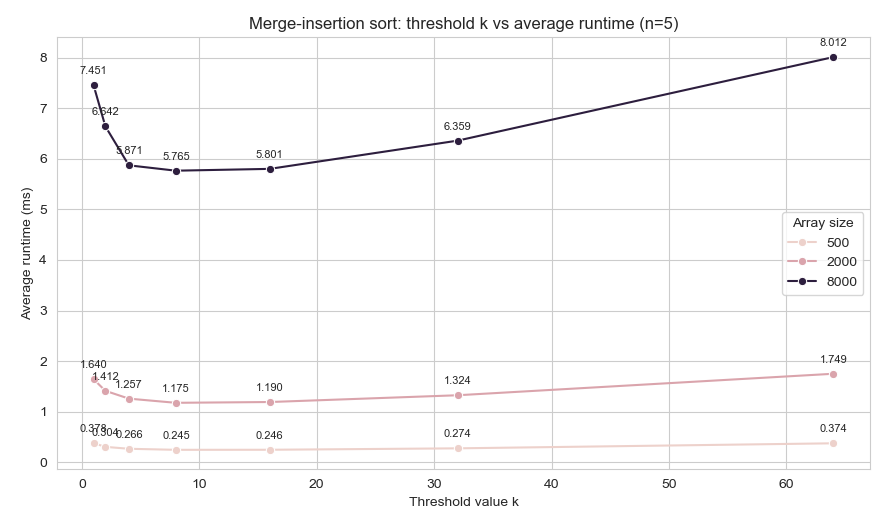
\includegraphics[width=0.95\textwidth]{assets_HW2/P2.png}
    \label{fig:hybrid_sort}
\end{figure}


\begin{enumerate}
    \item The code to generate this plot is included in the Github link at the top of this page. Checkout \textbf{HW2/problem2.py} for the code.
    \item The optimal value of $k$ in each problem size is $k=8$. In $N=500$, the average runtime at this threshold is $0.245$ ms. In $N=2000$, the average runtime at this threshold is $1.175$ ms. In $N=8000$, the average runtime at this threshold is $5.765$ ms.
    \item In merge sort, as we get deeper into the tree, more recursive calls are required. For every level of the the merge sort tree, we need double the number of recursive calls as compared to the previous level. At low values of $k$, since the threshold is so low, we practically have to traverse the merge sort tree to almost the same number of tree levels as the un-modified merge sort tree. This means that we do not really save that many recursive calls. At high values of $k$, the inefficency of the insertion sort algorithm overpowers the overhead of the recursive calls from merge sort. In this case, we do not traverse many levels of the merge sort tree, and the inefficent merge sort is applied on relatviely large paritions of the array.
\end{enumerate}


% Problem 3 - Counting Inversions
\begin{problem}{}{problem-3}
    An \textbf{inversion} in an array is a pair of indices $(i, j)$ where $i < j$ but $\texttt{arr}[i] > \texttt{arr}[j]$. This measures ``how unsorted'' an array is.

    \vspace{1ex}
    \noindent\textbf{Task:} Modify merge sort to count the total number of inversions in $O(n \log n)$ time.

    \vspace{1ex}
    \noindent\textbf{Examples:}
    \begin{itemize}
        \item $[1, 2, 3, 4]$ has 0 inversions (already sorted)
        \item $[4, 3, 2, 1]$ has 6 inversions (reverse sorted)
        \item $[2, 4, 1, 3]$ has 3 inversions: $(\texttt{arr}[0], \texttt{arr}[2]) = (2,1)$, $(\texttt{arr}[1], \texttt{arr}[2]) = (4,1)$, $(\texttt{arr}[1], \texttt{arr}[3]) = (4,3)$, where each pair shows indices $(i,j)$ with $i < j$ and $\texttt{arr}[i] > \texttt{arr}[j]$
    \end{itemize}

    \vspace{1ex}
    \noindent\textbf{Questions:}
    \begin{enumerate}
        \item What is the maximum number of inversions possible for an array of size $n$?
        \item How does the inversion count relate to sorting algorithms like bubble sort?
    \end{enumerate}

\end{problem}

\vspace{1ex}
\noindent\textbf{Implementation:}
\lstinputlisting[language=Python,caption={Merge sort with inversion counting (\texttt{problem3.py})}]{../HW2/problem3.py}

\vspace{0.5ex}
\noindent\textbf{Sample output:}
\begin{lstlisting}[numbers=none, frame=single, basicstyle=\ttfamily\small]
[1, 2, 3, 4] -> after merge sort: [1, 2, 3, 4] -> number of inversions = 0
[4, 3, 2, 1] -> after merge sort: [1, 2, 3, 4] -> number of inversions = 6
[2, 4, 1, 3] -> after merge sort: [1, 2, 3, 4] -> number of inversions = 3
\end{lstlisting}

\begin{enumerate}
    \item The maximum number of inversions possible for an array of size $n$ will come when the list is completely reversed. In this case the number of inversions for each element (starting from the last) will be the number of elements before it: $ (n-1) + (n-2) + ... + 1$. This can be simplified to: $$ \sum_{i=0}^{n-1} i = \frac{n(n-1)}{2} $$

    \item The inversion count is related to bubble sort (and other related sorting algorithms) because the number of inversions is equal to the number of swaps needed to sort the array in those algorithms.

\end{enumerate}


% Problem 4 - Queue Using Two Stacks
\begin{problem}{}{problem-4}
    Show how to implement a queue using two stacks.
\end{problem}

We can have two stacks, call one the \textbf{auxiliary stack} and the other the \textbf{main stack}. When inserting an element into the queue, pop all elements from the main stack and push them into the auxiliary stack, one by one. Then push the incoming element into the main stack. Then pop all the elements from the auxiliary stack and push then back into the main stack. This method preserves the order of the elements in a queue formation in the main stack. When we want to de-queue an element, we can pop the top element of the main stack.


% Problem 5 - Merge Two Sorted Linked Lists
\begin{problem}{}{problem-5}
    You are given the heads of two sorted linked lists \texttt{list1} and \texttt{list2}. Write a solution that merges the two lists into one sorted list. The list should be made by splicing together the nodes of the first two lists. Your function should return the head of the merged linked list.

    \vspace{1ex}
    \noindent\textbf{Example:}\\
    Input: \texttt{list1 = [1,2,4]}, \texttt{list2 = [1,3,4]}\\
    Output: \texttt{[1,1,2,3,4,4]}
\end{problem}

\vspace{1ex}
\noindent\textbf{Implementation:}
\lstinputlisting[language=Python,caption={Merge two sorted linked lists (\texttt{problem5.py})}]{../HW2/problem5.py}

\vspace{0.5ex}
\noindent\textbf{Sample output:}
\begin{lstlisting}[numbers=none, frame=single, basicstyle=\ttfamily\small]
inserting 1 from list2
inserting 1 from list1
inserting 2 from list1
inserting 3 from list2
inserting 4 from list2
1 -> 1 -> 2 -> 3 -> 4 -> 4 -> None
\end{lstlisting}


% Problem 6 - Sort Matrix Diagonals
\begin{problem}{}{problem-6}
    A \textbf{matrix diagonal} is a diagonal line of cells starting from some cell in either the topmost row or leftmost column and going in the bottom-right direction until reaching the matrix's end. Write a solution for a given $m \times n$ matrix of integers, sort each matrix diagonal in ascending order and return the resulting matrix.

    \vspace{1ex}
    \noindent\textbf{Example:}

    \[
    \text{Input:}
    \quad
    \begin{pmatrix}
    3 & 3 & 1 & 1 \\
    2 & 2 & 1 & 2 \\
    1 & 1 & 1 & 2
    \end{pmatrix}
    \qquad
    \text{Output:}
    \quad
    \begin{pmatrix}
    1 & 1 & 1 & 1 \\
    1 & 2 & 2 & 2 \\
    1 & 2 & 3 & 3
    \end{pmatrix}
    \]
\end{problem}

\vspace{1ex}
\noindent\textbf{Implementation:}
\lstinputlisting[language=Python,caption={Sort matrix diagonals (\texttt{problem6.py})}]{../HW2/problem6.py}

\vspace{0.5ex}
\noindent\textbf{Sample output:}
\begin{lstlisting}[numbers=none, frame=single, basicstyle=\ttfamily\small]
Original matrix:
[3, 3, 1, 1]
[2, 2, 1, 2]
[1, 1, 1, 2]
Sorted matrix:
[1, 1, 1, 1]
[1, 2, 2, 2]
[1, 2, 3, 3]
\end{lstlisting}


% Problem 7 - Binary Search Tree
\begin{problem}{}{problem-7}
    Consider the following sequence of numbers: $15, 10, 20, 8, 12, 17, 25$.

    \begin{enumerate}[(a)]
        \item Insert these numbers in the given order into a Binary Search Tree (BST). Draw the resulting tree.

        \item Identify whether the constructed BST is also a \textbf{Complete Binary Tree} and a \textbf{Full Binary Tree}. Justify your answer.

        \item What is the in-order traversal of the BST you constructed? What do you notice about the output?
    \end{enumerate}
\end{problem}

\begin{figure}[H]
    \centering
    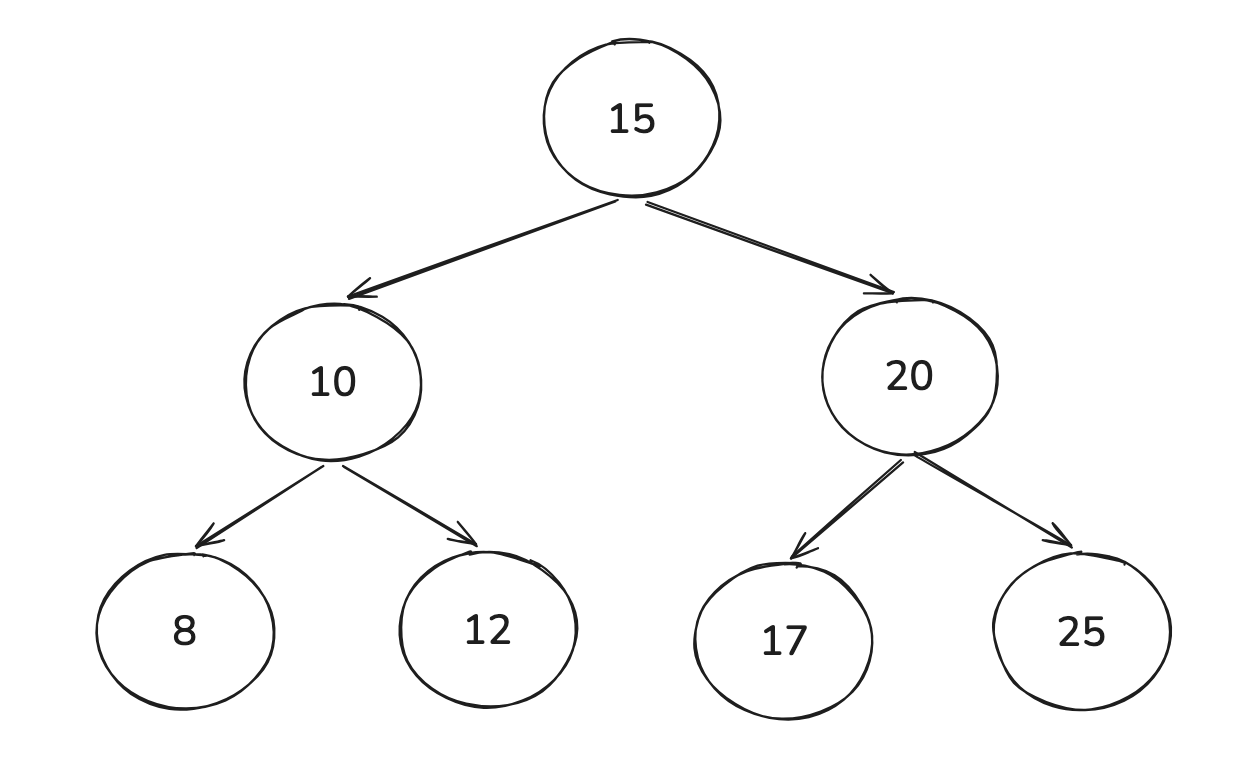
\includegraphics[width=0.7\textwidth]{assets_HW2/BST.png}
    \label{fig:bst}
\end{figure}

\begin{enumerate}
    \item The resulting tree is shown above.
    \item A \textbf{Full Binary Tree} is a binary tree in which all nodes are either completely filled or completely empty. The above binary tree is a full binary tree because all nodes show this behavior.
    \item A \textbf{Complete Binary Tree} is a binary tree in which all levels are completely filled except for the last level (left aligned). In the above tree, we see that all levels are completely filled; therefore, by default it is a complete binary tree.
    \item The in-order traversal of the BST is: $8, 10, 12, 15, 17, 20, 25$.
\end{enumerate}

\end{document}
